\chapter{Higher Dimensional Systems}

\subsection*{Section~\protect{\ref{sec:LinHomSys}} Linear Systems in Jordan
Normal Form}
\rhead{sec:LinHomSys}{LINEAR SYSTEMS IN JORDAN NORMAL FORM}

\exer{c11.1.1} \ans 
\[
X(t) =
\left(\begin{array}{c}
e^{2t}(t - 1) \\
e^{2t} \\
e^t(2\cos{t} + 3\sin{t}) \\
e^t(2\sin{t} - 3\cos{t})
\end{array}\right).
\]

\soln Write the system as the equation $\dot{X} = AX$, where
\[
A =
\left(\begin{array}{rrrr}
2 & 1 & 0 & 0 \\
0 & 2 & 0 & 0 \\
0 & 0 & 1 & -1 \\
0 & 0 & 1 & 1
\end{array}\right).
\]
Note that the matrix $A$ is in Jordan normal form, and has a double
eigenvalue at $\lambda = 2$ and a pair of complex conjugate eigenvalues
at $\lambda = 1 \pm i$.  Thus, we can compute the closed form solution
$X(t) = e^{At}X_0$ by computing the exponential of each Jordan block.  Let
\[
B = \mattwo{2}{1}{0}{2} \AND C = \mattwo{1}{-1}{1}{1}.
\]
Then, $B = 2I_2 + N$, where $N$ is the $2 \times 2$ matrix with an entry $1$
on the superdiagonal.  Since $I_2$ and $N$ commute,
\[
e^{Bt} = e^{2t}e^{tN} = e^{2t}(I_2 + tN) =
e^{2t}\mattwo{1}{t}{0}{1}.
\]
Since $C$ is a $2 \times 2$ block with complex eigenvalues, we can
compute its exponential as we have done in previous chapters, using
$\sigma = 1$ and $\tau = 1$:
\[
e^{Ct} = e^{\sigma t}\mattwo{\cos{(\tau t)}}{-\sin{(\tau t)}}
{\sin{(\tau t)}}{\cos{(\tau t)}}
= e^{t}\mattwo{\cos{t}}{-\sin{t}}{\sin{t}}{\cos{t}}.
\]
Thus,
\[
X(t) = e^{At}X_0 =
\left(\begin{array}{cccc}
e^{2t} & te^{2t} & 0 & 0 \\
0 & e^{2t} & 0 & 0 \\
0 & 0 & e^t\cos{t} & -e^t\sin{t} \\
0 & 0 & e^t\sin{t} & e^t\cos{t}
\end{array}\right)
\left(\begin{array}{r} -1 \\ 1 \\ 2 \\ -3 \end{array}\right)
= \left(\begin{array}{c}
e^{2t}(t - 1) \\
e^{2t} \\
e^t(2\cos{t} + 3\sin{t}) \\
e^t(2\sin{t} - 3\cos{t})
\end{array}\right).
\]

\exer{c11.1.3}  \ans $X(t) = \cvecthree{t + \frac{1}{2}t^2}{1 + t}{1}$. The distance from $X(0)$ to the 
origin is $\sqrt{2} \approx 1.4142$ and the distance from $X(2)$ to the origin is
$e^{-1}\sqrt{26} \approx 1.8758$.

\soln Let $B$ be the matrix of this system.  Note that $B$ is a single Jordan block
with a triple eigenvalue at $\lambda = -\frac{1}{2}$, and that we can write
$B = -\frac{1}{2}I_3 + N$, where $N$ is the matrix with entries $1$ on the
superdiagonal.  Then, since $I_3$ and $N$ commute, we can write:
\[
\begin{array}{rcl}
X(t) & = & e^{tB}X_0 \\
& = & e^{\lambda tI_3}e^{tN}X_0 \\
& = & e^{\lambda t}(I_3 + tN + \frac{1}{2}t^2N^2)X_0 \\
& = & e^{-\frac{1}{2} t}\cmatthree{1}{t}{\frac{1}{2}t^2}{0}{1}{t}{0}{0}{1}
\vecthree{0}{1}{1} \\
& = & \cvecthree{t + \frac{1}{2}t^2}{1 + t}{1}.
\end{array}
\]
Next, compute $X(2) = e^{-1}(4,3,1)^t$.
The distance from $X(0)$ to the origin is $\sqrt{0 + 1 + 1} = \sqrt{2}
\approx 1.4142$.  The distance from $X(2)$ to the origin is
$e^{-1}\sqrt{4^2 + 3^2 + 1} = e^{-1}\sqrt{26} \approx 1.8758$.
Thus, $X(2)$ is indeed further from the origin than $X(0)$.

\exer{c11.1.3B}  The differential equation $\dot{X}=JX$, where $J$ is the 
single Jordan block $4\times 4$ matrix with double eigenvalues $i$ and $-i$,
is:
\[
\dot{X} = \left(\begin{array}{rr|rr}
 0 & -1 & 1 &  0 \\
 1 &  0 & 0 &  1 \\
\hline
 0 &  0 & 0 & -1\\
 0 &  0 & 1 &  0
\end{array}\right)X.  
\]
Solutions to this differential equation are:
\[
X(t) = e^{tJ}X_0 = \left(\begin{array}{rrrr}
  \cos t & -\sin t & t\cos t & -t\sin t\\
  \sin t &  \cos t & t\sin t &  t\cos t\\
     0   &    0    &  \cos t &  -\sin t\\
     0   &    0    &  \sin t &   \cos t  
\end{array}\right)
\left(\begin{array}{r} x_1^0 \\  x_2^0 \\ x_3^0 \\ x_4^0 \end{array}\right)
\]
The first two coordinates of this solution are:
\begin{eqnarray*}
x_1(t) & = & x_1^0\cos t - x_2^0\sin t + x_3^0t\cos t - x_4^0t\sin t\\
x_2(t) & = & x_1^0\sin t + x_2^0\cos t + x_3^0t\sin t + x_4^0t\cos t
\end{eqnarray*}
We can rewrite these coordinates in vector form as:
\[
\vectwo{x_1(t)}{x_2(t)} =
(x_1^0 + tx_3^0t)\vectwo{\cos t}{\sin t} + 
(x_2^0 + tx_4^0t)\vectwo{-\sin t}{\cos t}.
\] 
As long as either $x_3^0\neq 0$ or $x_4^0\neq 0$, the solution will spiral 
away from the origin (as seen by its projection in the $x_1x_2$ plane) in 
both forward and backward time.

\exer{c11.1.7}  
\ans $e^{tJ}= \cmattwo{e^{-t}\left(\begin{array}{rrr} 
 1 & t & \frac{1}{2}t^2\\ 0 & 1 & t\\ 0 & 0 & 1\end{array}\right)}{0}{0}
{e^{2t}\mattwo{1}{t}{0}{1}}$.

\soln Since $J$ is a block form
\[
J = \left(\begin{array}{rrr|rr} 
-1 &  1 &  0 &  0 & 0 \\ 
 0 & -1 &  1 &  0 & 0 \\
 0 &  0 & -1 &  0 & 0 \\
\hline
 0 &  0 &  0 &  2 & 1 \\
 0 &  0 &  0 &  0 & 2
\end{array}\right)
\]
Jordan form matrix, we can exponentiate the diagonal blocks separately.

\exer{c11.1.5A}
\ans $X(t) = e^t\left(\begin{array}{rrr}
     3  &  -4   &   1\\
    -6   &  11   &   0\\
    15   & -32   &   0 \end{array}\right)
\left(\begin{array}{rrr}
     1  &  t   &   \frac{1}{2}t^2\\
    0   &  1   &   t\\
    0   &  0   &   1 \end{array}\right)
\left(\begin{array}{r} 0.4074\\ 0.2222\\ 0.6667\end{array}\right)$.

\vspace{0.08in}

\soln  In \Matlabp, load the matrix $A$ and the initial vector $X_0$. 
Begin by finding the eigenvalues of $A$ by typing {\tt eig(A)} and
obtaining
\begin{verbatim}
ans =
   1.0000          
   1.0000 + 0.0000i
   1.0000 - 0.0000i
\end{verbatim}
So $1$ is an eigenvalue of $A$ of multiplicity three.  To find the Jordan
block structure of $A$ type {\tt null(A-eye(3))} obtaining
\begin{verbatim}
ans =
    0.1826
   -0.3651
    0.9129
\end{verbatim}
Thus, the Jordan normal form of $A$ is 
\[
J = \left(\begin{array}{rrr} 1 & 1 & 0\\ 0 & 1 & 1\\ 0 & 0 & 1 
\end{array}\right).
\]
The solution to the differential equation is:
\[
X(t) = e^{tA}X_0 = e^{tSJS\inv}X_0= Se^{tJ}S\inv X_0.
\]
where $J=S\inv AS$.  To compute the matrix $S$ we need to choose a vector 
$v_3$ that is in $\R^3\setmin\nulls(A-I_3)^2$.  The vector $v_3=e_3$ will
work. Then type the commands
\begin{verbatim}
v3 = [1 0 0]';
v2 = (A-eye(3))*v2;
v1 = (A-eye(3))*v2;
S  = [v1 v2 v3]
\end{verbatim}
obtaining
\begin{verbatim}
S =
     3    -4     1
    -6    11     0
    15   -32     0
\end{verbatim}
To check that we have derived the correct matrix type {\tt inv(S)*A*S}
and obtain
\begin{verbatim}
ans =
    1.0000    1.0000    0.0000
   -0.0000    1.0000    1.0000
   -0.0000    0.0000    1.0000
\end{verbatim}
It follows that the solution is:
\[
X(t) = Se^{tJ}S\inv X_0 = e^t\left(\begin{array}{rrr}
     3  &  -4   &   1\\
    -6   &  11   &   0\\
    15   & -32   &   0 \end{array}\right)
\left(\begin{array}{rrr}
     1  &  t   &   \frac{1}{2}t^2\\
    0   &  1   &   t\\
    0   &  0   &   1 \end{array}\right)
\left(\begin{array}{r} 0.4074\\ 0.2222\\ 0.6667\end{array}\right)
\] 
where $S\inv X_0$ is calculated by typing {\tt inv(S)*X0}.

\exer{c11.1.6A} \ans Solutions are linear combinations of the functions 
$e^{5t}$ and $t^je^t$ for $j=0,1,2$.

\soln In \Matlabp, load the matrix $A$.  Begin by 
finding the eigenvalues of $A$ by typing {\tt eig(A)} and obtaining
\begin{verbatim}
ans =
   5.0000          
   0.9999          
   1.0000 + 0.0001i
   1.0000 - 0.0001i
\end{verbatim}
Because of numerical errors there may be some confusion.  The eigenvalues of
$A$ are $1$ with multiplicity three and $5$ with multiplicity one.  Next,
find the Jordan block structure corresponding to the eigenvalue $1$ by typing
{\tt null(A-eye(4))} and obtaining
\begin{verbatim}
ans =
   -0.9733
    0.2141
    0.0584
    0.0584
\end{verbatim}
Therefore, there is one Jordan block associated to the eigenvalue $1$.  The
solutions to the associated linear differential equation are linear
combinations of the functions $e^{5t}$, $e^t$, $te^t$, and $t^2e^t$.



\subsection*{Section~\protect{\ref{S:QT}} Qualitative Theory Near Equilibria}
\rhead{S:QT}{QUALITATIVE THEORY NEAR EQUILIBRIA}


\exer{c14.2.1A} \ans $\left(\begin{array}{rrr}
-10 & -2 & -1\\ 9 & 1 & 4 \\ -14 & 20 & 1\end{array}\right)$.

\vspace{0.08in}

\soln  The Jacobian matrix is
\[
J(x,y,z) = \left(\begin{array}{ccc}
2 - 6x & 2y & -1\\ 1+2z & 1 & 2x\\ 10y-2x & 10x & 1\end{array}\right).
\]
Evaluating at $(x,y,z)=(2,-1,4)$ yields the answer.

\exer{c14.2.1C} \ans The origin is not stable.

\soln The eigenvalues of $J(2,-1,4)$ are
\begin{verbatim}
  -4.2656 + 7.5182i
  -4.2656 - 7.5182i
   6.5312          
\end{verbatim}
Since there is a positive eigenvalue, the equilibrium is not 
asymptotically stable.


\newpage
\exer{c14.2.1E} \ans There are two equilibria $(1,1,1)$ and $(3,-3,9)$.
The equilibium $(1,1,1)$ has three unstable directions while the
equilibrium $(3,-3,9)$ has two unstable directions and one stable directions.

\soln  Finding the equilibria is done by solving the equations
\begin{eqnarray*}
x^2-z & = & 0 \\
y^2-z & = & 0 \\
2x+y-3 & = & 0.
\end{eqnarray*}
The first two equations imply that $x^2=y^2$.  Hence $x=y$ or $x=-y$. 
Substituting into the third equation allows us to find the two equilibria
$(1,1,1)$ and $(3,-3,9)$.  Next, compute the Jacobian matrix
\[
J(x,y,z) = \left(\begin{array}{ccc}
2x & 0 & -1\\ 0 & 2y & -1\\ 2 & 1 & 0 \end{array}\right).
\]
Evaluating at the equilibria yields the matrices
\[
J(1,1,1) = \left(\begin{array}{ccc}
2 & 0 & -1\\ 0 & 2 & -1\\ 2 & 1 & 0 \end{array}\right)
\AND 
J(3,-3,9) = \left(\begin{array}{ccc}
6 & 0 & -1\\ 0 & 6 & -1\\ 2 & 1 & 0 \end{array}\right).
\]
The eigenvalues of $J(1,1,1)$ are
\begin{verbatim}
   1.0000 + 1.4142i
   1.0000 - 1.4142i
   2.0000     
\end{verbatim}
and the eigenvalues of $J(3,-3,9)$ are
\begin{verbatim}
    5.6514
    0.1820
   -5.8334
\end{verbatim}
The equilibium $(1,1,1)$ has three unstable directions while the
equilibrium $(3,-3,9)$ has two unstable directions and one stable 
directions.

\exer{c11.2.1a}
\ans The origin is an asymptotically stable equilibrium.

\soln Using \Matlabp, find that the eigenvalues of $C$ are $\lambda_1
\approx -0.2679$ and $\lambda_2 \approx -3.7321$.  Both eigenvalues
have negative real part, so the origin is asymptotically stable.

\exer{c11.2.1c}
\ans The origin is an asymptotically stable equilibrium.

\soln The eigenvalues of $C$ are $-0.5 \pm 0.2i$, $-0.2$, and $-0.1$, all
of which have negative real part.

\exer{c11.2.2b} \ans There are four unstable directions and one stable 
direction.

\soln  In \Matlabp, load the matrix $C$.  Find the eigenvalues of $C$ by
typing {\tt eig(C)} obtaining
\begin{verbatim}
ans =
  -0.4516          
   2.2585 + 4.3244i
   2.2585 - 4.3244i
  13.7788          
  10.1559   
\end{verbatim}
Therefore, there are four unstable directions and one stable direction.



\subsection*{Section~\protect{\ref{S:ode45}} \Matlab {\tt ode45} in One Dimension}
\rhead{S:ode45}{MATLAB {\tt ode45} IN ONE DIMENSION}

\exer{c11.3.2a}
Create the file {\tt exode3\_1.m} containing the text
\begin{verbatim}
function f1 = exode3_1(t)
f1 = sin(t) - t^3;
\end{verbatim}

\exer{c11.3.2c}
Create the file {\tt exode3\_3.m} containing the text
\begin{verbatim}
function f3 = exode3_3(x,y)
f3 = [x*y - 1, x + 2*y];
\end{verbatim}

\exer{c11.3.2e}
Create the file {\tt exode3\_5.m} containing the text
\begin{verbatim}
function f5 = exode3_5(u)
f5 = [u(1) - 2*u(3); u(1)*u(2)*u(3)];
\end{verbatim}

\exer{c11.3.2A}
To show that $y(t)=e^{(t^2-4)/2}$ is a solution to the differential equation
$\dot{x}=tx$ with initial value $x(2)=1$, evaluate $y(2)=e^0=1$ and
differentiate
\[
\frac{dy}{dt} = e^{(t^2-4)/2}\frac{d}{dt}((t^2-4)/2) = 
e^{(t^2-4)/2}t = ty.
\]

To establish the accuracy of {\tt ode45} numerically, begin by creating the 
m-file to evaluate $f(t,x)=tx)$:
\begin{verbatim}
function f = ftx(t,x)
f = t*x;
\end{verbatim}
Then set the options in {\sf ode45} so that the absolute and relative
tolerances are at $10^{-6}$:
\begin{verbatim}
options = odeset('RelTol',1e-6,'AbsTol',1e-6);
\end{verbatim}
Then integrate the differential equation with the commands:
\begin{verbatim}
tspan = 2:0.01:3;
[t,x] = ode45('ftx',tspan,[1],options);
\end{verbatim}
The graph of $x(t)$ obtained by typing {\tt plot(t,x)} is shown in
Figure~\ref{c11.3.2A}a.  The plot of the theoretically exact solution
is shown in Figure~\ref{c11.3.2A}b and is obtained by typing
\begin{verbatim}
clf
y = exp((t.^2-4)/2);
plot(t,y)
\end{verbatim}
Note that the two figures are identical.  To evaluate $x(2.5)$ and $x(2.75)$,
note that {\tt t(51) = 2.5} and {\tt t(76) = 2.75}.  Using {\tt format long}, 
we evaluate {\tt x(51)}, {\tt y(51)}, {\tt x(76)}, {\tt y(76)} obtaining
\begin{verbatim}
x(51) = 3.08021795611640  and  y(51) = 3.08021684891803
x(76) = 5.93727630788575  and  y(76) = 5.93727337374561
\end{verbatim}
Note that the two function values are equal to an error of less than 
$10^{-5}$.

\begin{figure}[htb]
     \centerline{%
     \psfig{file=exfigure/fig3_8a.eps,width=2.75in}
     \psfig{file=exfigure/fig3_8b.eps,width=2.75in}}
	\exercaptwo{c11.3.2A}
\end{figure} 



\subsection*{Section~\protect{\ref{S:ode45HD}} Higher Dimensional Systems Using 
{\tt ode45}}
\rhead{S:ode45HD}{HIGHER DIMENSIONAL SYSTEMS USING {\tt ode45}}

\exer{c11.3.1a}
\ans The origin is a stable equilibrium.

\soln Create the following m-file to define the function {\tt exode4\_1}:
\begin{verbatim}
function f=exode4_1(t,x)
A = [-5     1    -3     0
     -2     3    -3     0
      4    11    -5     0
      2    -5     3    -2];
f = A*x;
\end{verbatim}
Compute the eigenvalues of $A$.  In this case, $\lambda_1 = -2$, $\lambda_2
\approx -0.25$, $\lambda_3 \approx -3.38 + 5.38i$, and $\lambda_4 \approx
-3.38 - 5.38i$ are eigenvalues of $A$.  All four eigenvalues have negative
real part, so the origin is a stable equilibrium.

\para To view the system using {\tt ode45}, choose an initial vector $X_0$
near the origin, and run {\tt ode45} using this vector.  Graphing the
components of the resulting $x$ confirms that all components converge on $0$
in forward time.  For example, the command
\begin{verbatim}
[t,x]=ode45('exode1',[0 5],[1,1,1,1]');
\end{verbatim}
runs {\tt ode45} on the system with initial vector $X_0 = (1,1,1,1)^t$.
The trajectories of the components of $x$ are shown in Figure~\ref{c11.3.1a}.

\begin{figure}[htb]
                       \centerline{%
                       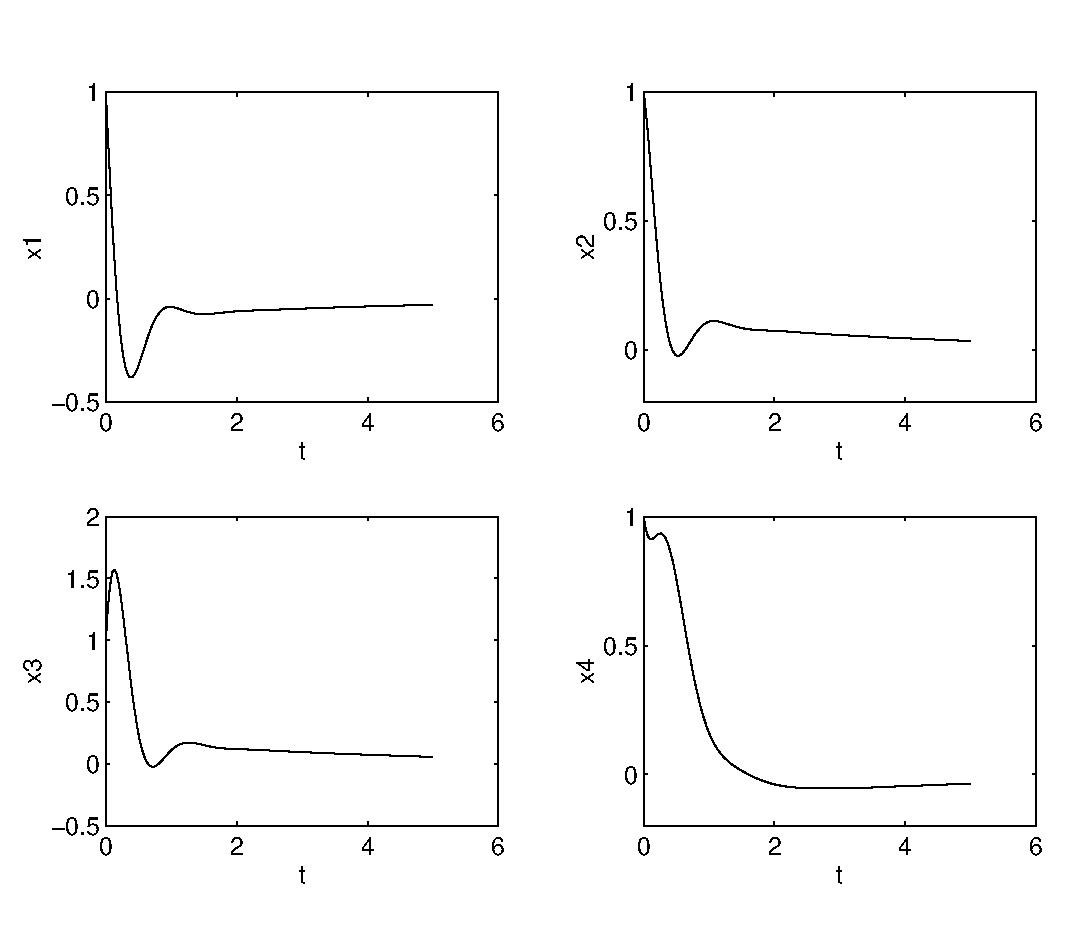
\psfig{file=exfigure/11-3-1a.eps,width=3.0in}}
                \exercap{c11.3.1a}
\end{figure}

\exer{c11.4.1a}  The origin is asymptotically stable. 

\exer{c11.4.1c}  The equilibrium $(1,0,2)$ is not asymptotically stable. 

\exer{c11.4.7}  Computer experiment.



\subsection*{Section~\protect{\ref{S:NLD}} Quasiperiodic Motions and Tori}
\rhead{S:NLD}{QUASIPERIODIC MOTIONS AND TORI}

\exer{EX:tor4}
(a) Let {\tt X0} be an initial condition of your choice, written as a
column vector.  Then the command {\tt [t,x]=ode45('ftor4',0,100,X0)}
will find solutions to the system $\dot{X} = AX$ with initial condition
$X_0$.  For most choices of $X_0$, the graphs are similar to those shown
in Figures~\ref{F:ftor4ts} and \ref{F:ftorphase} in the text.

(b) Load matrix $A$ into \Matlabp.  Then, use the command
{\tt [S,D] = eig(A)} to find that $\lambda = 4.7958i$ is an eigenvalue of
$A$ with corresponding eigenvector $v = (-0.3447 + 0.7587i, 0.0139 +
0.3724i, 0.0800 + 0.1462i, 0.0139 + 0.03724i)$.  Using {\tt ode45}, find
the solutions to the system with initial condition $X_0 = (-0.3447, 0.0139,
0.0800, 0.0139)^t$.  The time series of this system are shown in
Figure~\ref{EX:tor4}a, and three phase portraits are shown in
Figure~\ref{EX:tor4}b.

\begin{figure}[htb]
                       \centerline{%
                       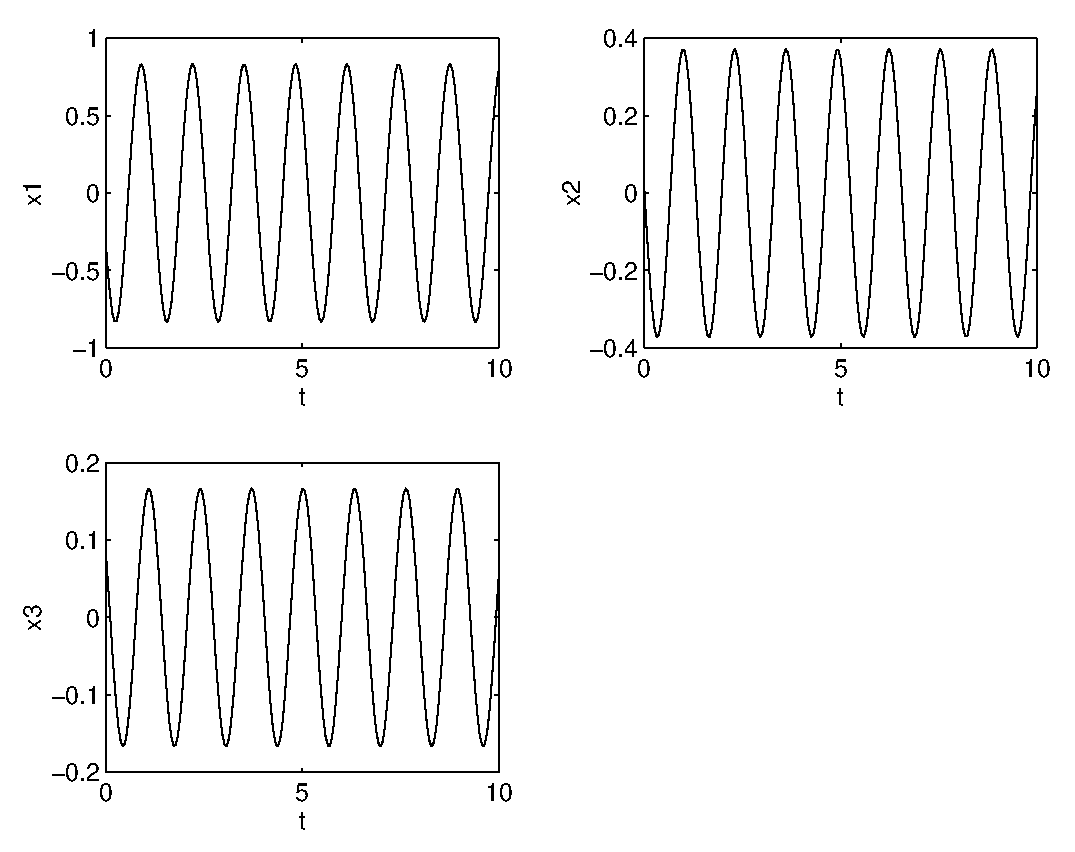
\psfig{file=exfigure/tor4a.eps,width=2.0in}
			\hspace{1.0in}
                       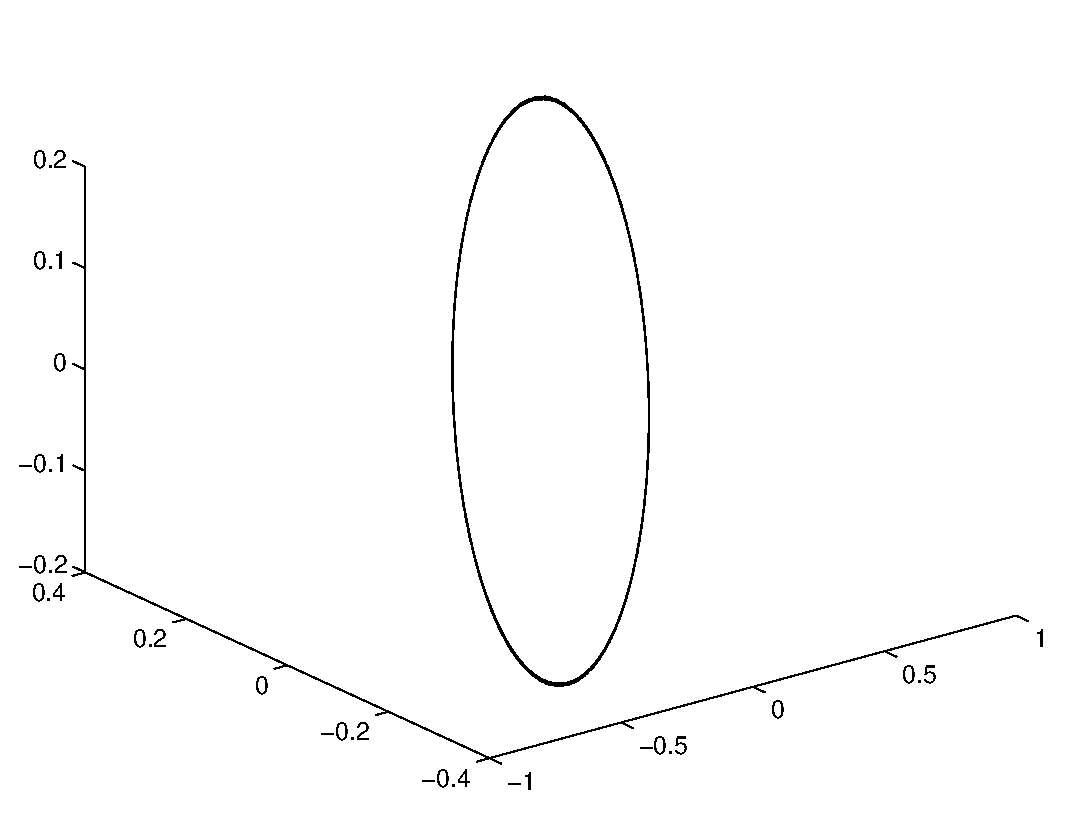
\psfig{file=exfigure/tor4b.eps,width=2.0in}}
                \exercaptwo{EX:tor4}
\end{figure}

\exer{c14.5.2b} \ans No.

\soln The eigenvalues of $A$ are 
\begin{verbatim}
  -0.5104 + 4.5851i
  -0.5104 - 4.5851i
   0.5104 + 1.8703i
   0.5104 - 1.8703i
\end{verbatim}
The eigenvalues are not purely imaginary.

\exer{c14.5.2d} \ans No.

\soln The eigenvalues of $A$ are 
\begin{verbatim}
  -0.9999 + 2.9587i
  -0.9999 - 2.9587i
   0.2677          
   3.7321          
  -1.0000          
\end{verbatim}
The eigenvalues are not purely imaginary.



\newpage
\subsection*{Section~\protect{\ref{S:chaos}} Chaos and the Lorenz Equation}
\rhead{S:chaos}{CHAOS AND THE LORENZ EQUATION}

\exer{c11.4.1} \ans The system has unstable equilibria $X_1 = (0,0,0)$, 
$X_2 = (6\sqrt{2},6\sqrt{2},27)$, and $X_3 = (-6\sqrt{2},-6\sqrt{2},27)$.

\soln The equilibria of the system occur when $\dot{x_1} = 0$, $\dot{x_2}
= 0$, and $\dot{x_3} = 0$.  According to the first equation of the Lorenz
system, $\dot{x_1} = 0$ when $x_1 = x_2$.  Thus, at the equilibria, the
other two equations can be rewritten
\[
\begin{array}{rcl}
0 & = & \dot{x_2} = \rho x_1 - x_1 - x_1x_3 = x_1(\rho - 1 - x_3). \\
0 & = & \dot{x_3} = -\beta x_3 + x_1^2. \\
\end{array}
\]
So, the system is in equilibrium either at the origin, $X =
(\sqrt{\beta (\rho - 1)}, \sqrt{\beta (\rho - 1)}, \rho 1)$, or
$X = (-\sqrt{\beta (\rho - 1)}, -\sqrt{\beta (\rho - 1)}, \rho - 1)$.
To compute the stabilities at the equilibria, first find the general
Jacobian matrix for the system:
\[
dJ = \cmatthree{-\sigma}{\sigma}{0}{\rho - x_3}{-1}{-x_1}{x_2}{x_1}{-\beta}.
\]
Substitute in the values $\beta = -\frac{8}{3}$, $\rho = 28$, and $\sigma
= 10$ to obtain
\[
dJ = \cmatthree{-10}{10}{0}{28 - x_3}{-1}{-x_1}{x_2}{x_1}{-\frac{8}{3}}
\]
and $X_1 = (0,0,0)$, $X_2 = (6\sqrt{2},6\sqrt{2},27)$, and
$X_3 = (-6\sqrt{2},-6\sqrt{2},27)$.  Then compute the eigenvalues at the
equilibria.  At $X_1$, there are two negative real eigenvalues and one 
positive real eigenvalue, so $X_1$ cannot be stable.  At $X_2$ and $X_3$,
there is one negative real eigenvalue and a pair of complex conjugate
eigenvalues with positive real part.  Determine numerically that most
initial conditions do not converge on either $X_2$ or $X_3$ in forward time,
so $X_2$ and $X_3$ are not stable.

\exer{c11.4.3}
\ans The system has unstable equilibria at $X_1 = (0,0,0)$,
$X_2 = (\sqrt{60},0, -\sqrt{60})$, and $X_3 = (-\sqrt{60},0,\sqrt{60})$.
Figure~\ref{c11.4.3}a shows the behavior of $x$, $y$, and $z$ as $t$
increases.  Figure~\ref{c11.4.3}b shows the graph of the system created
with the {\tt plot3} command.  Figure~\ref{c11.4.3}c shows the same graph
with an overhead view of the $xz$ plane, and with circles indicating the
locations of the equilibria.  In forward time, trajectories oscillate
between circuits around the two nonzero equilibria.

\soln Find the equilibria by finding the points at which $\dot{x} = 0$,
$\dot{y} = 0$, and $\dot{z} = 0$.  Then, compute the general Jacobian
matrix
\[
dJ = \cmatthree{\alpha(-m_0 - m_1x^2)}{\alpha}{0}{1}{-1}{1}{0}{-\beta}{0}
= \cmatthree{-9 - 0.01x^2}{18}{0}{1}{-1}{1}{0}{-33}{0}.
\]
To see that the equilibria are unstable, find the Jacobian matrices at
each equilibrium.  Also note that most trajectories do not converge on
any of the equilibria in forward time.

\begin{figure}[htb]
                       \centerline{%
                       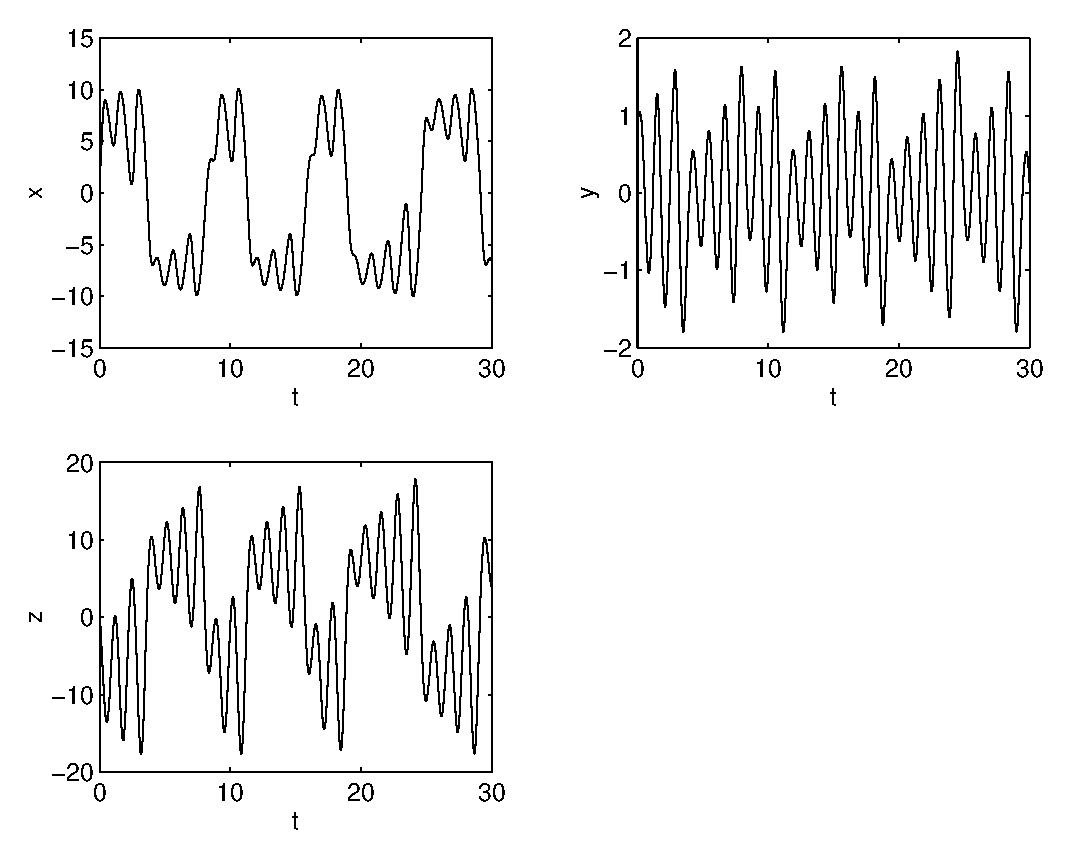
\psfig{file=exfigure/11-4-3a.eps,width=1.35in}
			\hspace{0.5in}
                       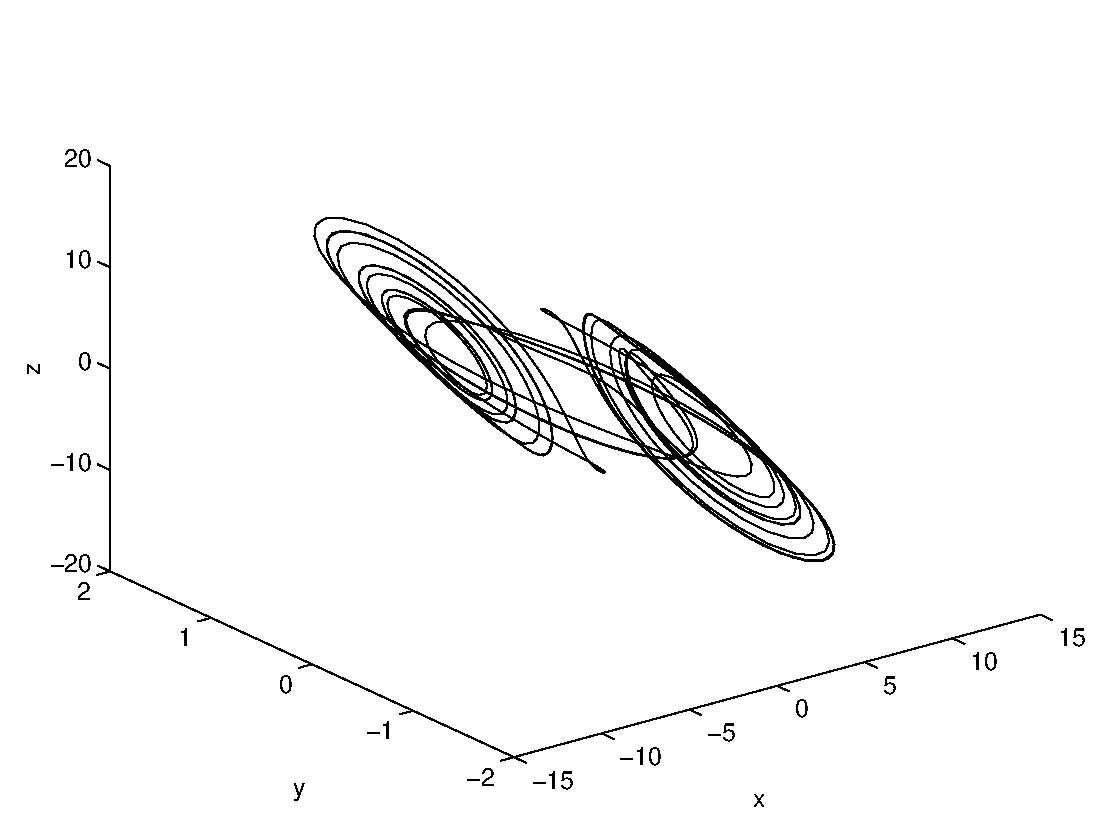
\psfig{file=exfigure/11-4-3b.eps,width=1.35in}
			\hspace{0.3in}
                       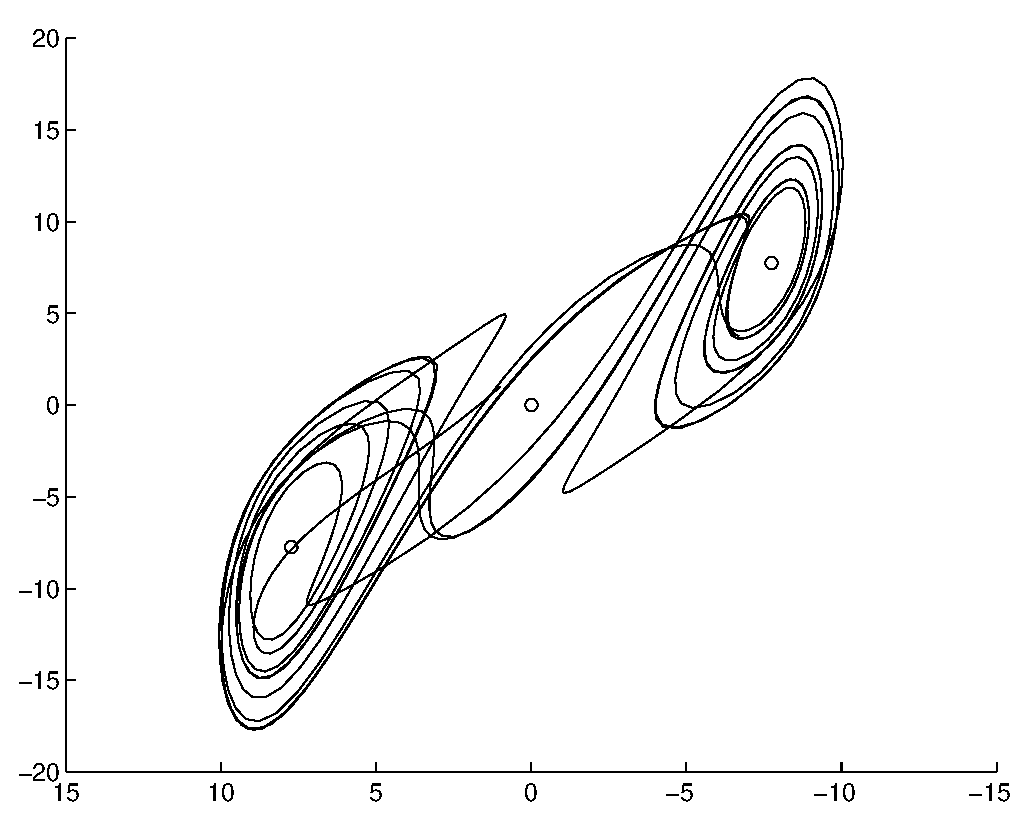
\psfig{file=exfigure/11-4-3c.eps,width=1.35in}}
		\exercapthree{c11.4.3}
\end{figure}

\exer{c11.6.1a} \ans The solution is asymptotic to an equilibrium.

\soln Solve the system using the m-file:
\begin{verbatim}
function f = f14_6_5(t,x)
f = [1 - x(1) - x(2)*x(2); -x(2) - x(3)*x(3); x(3) + x(1)*x(2) - x(3)^3];
\end{verbatim}

Compute the solution using \Matlab as follows:
\begin{verbatim}
[t,x] = ode45('f14_6_5',[0,40],[0.1, 0.2, 0.25]');
\end{verbatim}
\begin{figure}[htb]
     \centerline{%
     \psfig{file=exfigure/figf14_6_2.eps,width=3.5in}}
	\exercap{c11.6.1a}
\end{figure}
The time series are given in Figure~\ref{c11.6.1a} and show
that each coordinate function is eventually constant.  So the asymptotic
solution is an equilibrium.

\exer{c11.6.1c} \ans The solution is a new form of asymptotic behavior.

\soln Solve the system  using the m-file:
\begin{verbatim}
function f = f14_6_7(t,x)
a= 1.0; b = 1.5; c = 0.6;
f = [x(1) - (a*x(1)^2 + b*x(2)^2 + c*x(3)^2)*x(1) 
        x(2) - (c*x(1)^2 + a*x(2)^2 + b*x(3)^2)*x(2)
        x(3) - (b*x(1)^2 + c*x(2)^2 + a*x(3)^2)*x(3)];
\end{verbatim}
Compute the solution using \Matlab as follows:
\begin{verbatim}
[t,x] = ode45('f14_6_7',[0,1000],[0.10, 0.23, 0.15]');
\end{verbatim}

The time series in Figure~\ref{c11.6.1c}a never settle down but approach in 
order three separate
equilibria.  The solution is asymptotic to a cycle of heteroclinic
trajectories and is a new form of asymptotic behavior.  The three 
dimensional plot of the asymptotic solution is obtained by typing
\begin{verbatim}
size(t)
\end{verbatim}
obtaining
\begin{verbatim}
ans =
        2749           1
\end{verbatim}
and then typing
\begin{verbatim}
s = 500:1:2749;
plot3(x(s,1),x(s,2),x(s,3))
\end{verbatim}
The cycle of heteroclinic orbits is shown in Figure~\ref{c11.6.1c}b.

\begin{figure}[htb]
     \centerline{%
     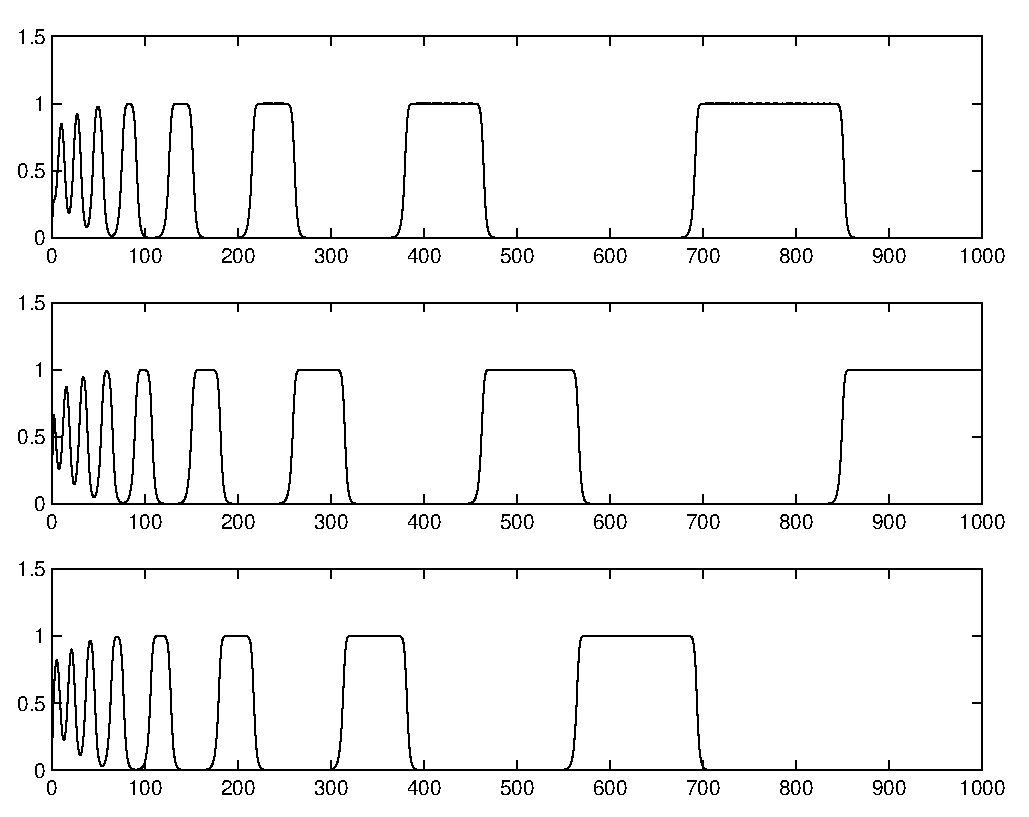
\psfig{file=exfigure/figf14_6_4.eps,width=2.7in}
     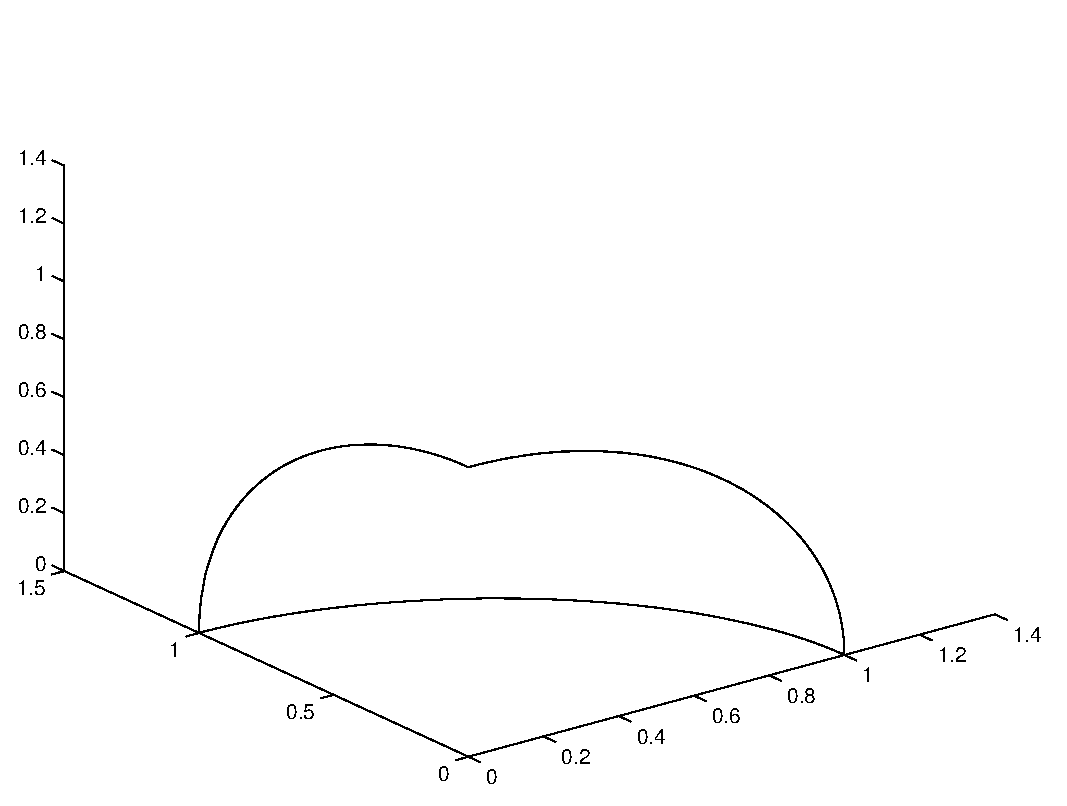
\psfig{file=exfigure/figf14_6_4a.eps,width=2.7in}}
	\exercaptwo{c11.6.1c}
\end{figure}


\newpage
\exer{c11.6.1e}  \ans The asymptotic dynamics of this solution is chaotic.

\soln Solve the system using the m-file:
\begin{verbatim}
function f = f14_6_9(t,x)
a = 5.7; b = 0.2; c = 0.2;
f = [-x(2)-x(3); 
     x(1) + b*x(2); 
     c + x(3)*(x(1)-a)];
\end{verbatim}

Compute the solution using \Matlab as follows:
\begin{verbatim}
[t,x] = ode45('f14_6_9',[0,400],[0.10, 0.11, 0.15]');
\end{verbatim}
This integration takes awhile.  The three dimensional plot of the
solution is given in Figure~\ref{c11.6.1e}.  Note the complicated behavior
reminiscent of the Lorenz equations.  The asymptotic dynamics of this
solution is chaotic.  Sensitive dependence on initial conditions can be
checked.

\begin{figure}[htb]
     \centerline{%
     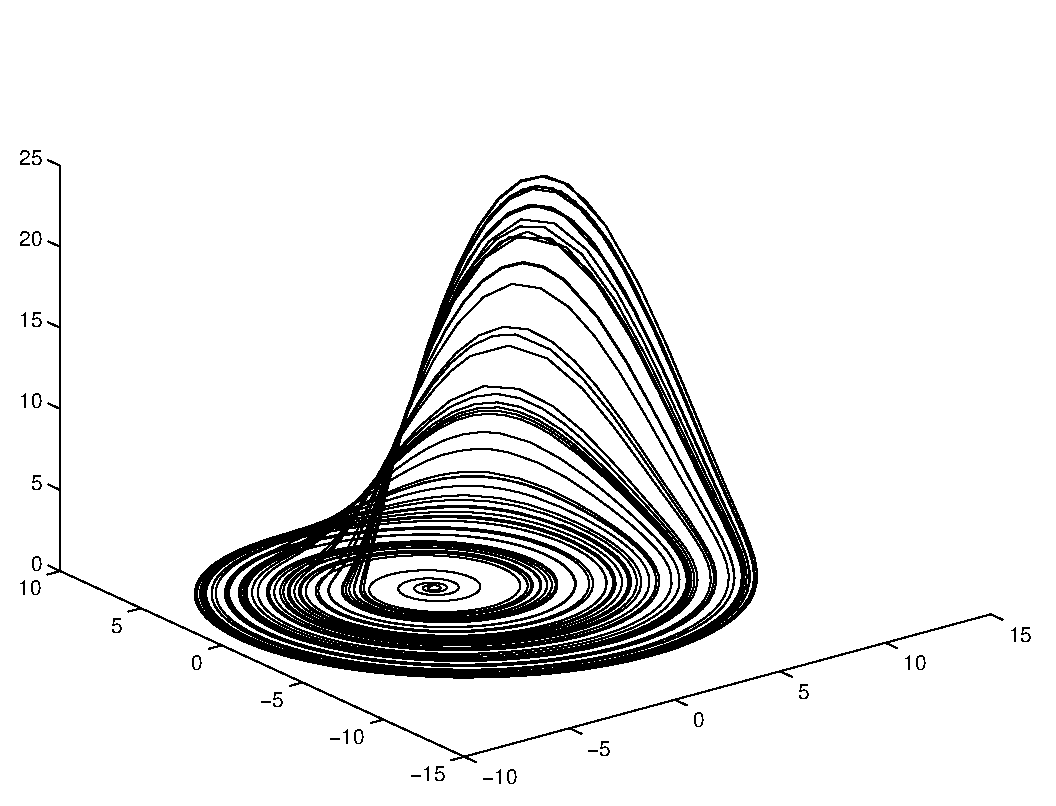
\psfig{file=exfigure/figf14_6_6.eps,width=3.0in}}
	\exercap{c11.6.1e}
\end{figure} 

\exer{c11.6.1f} \ans The solution is asymptotic to a periodic solution.

\soln Solve the system using the m-file:
\begin{verbatim}
function f = f14_6_11(t,x)
a = 1; b = 0.2; c = 0.2;
f = [-x(2)-x(3); 
     x(1) + b*x(2); 
     c + x(3)*(x(1)-a)];
\end{verbatim}

Compute the solution using \Matlab as follows:
\begin{verbatim}
[t,x] = ode45('f14_6_11',[0,80],[2.0, 0.5, 1.0]');
\end{verbatim}
The time series plot in Figure~\ref{c11.6.1f} shows convergence to a periodic solution.  

\begin{figure}[htb]
     \centerline{%
     \psfig{file=exfigure/figf14_6_8.eps,width=3.0in}}
	\exercap{c11.6.1f}
\end{figure} 

















